%% LyX 1.3 created this file.  For more info, see http://www.lyx.org/.
%% Do not edit unless you really know what you are doing.
\documentclass[english, 12pt]{article}
\usepackage{times}
%\usepackage{algorithm2e}
\usepackage{url}
\usepackage{bbm}
\usepackage[T1]{fontenc}
\usepackage[latin1]{inputenc}
\usepackage{geometry}
\geometry{verbose,letterpaper,tmargin=2cm,bmargin=2cm,lmargin=1.5cm,rmargin=1.5cm}
\usepackage{rotating}
\usepackage{color}
\usepackage{graphicx}
\usepackage{amsmath, amsthm, amssymb}
\usepackage{setspace}
\usepackage{lineno}
\usepackage{hyperref}
\usepackage{bbm}
\usepackage{makecell}

%\renewcommand{\arraystretch}{1.8}

%\usepackage{xr}
%\externaldocument{paper-ldpred2-supp}

%\linenumbers
%\doublespacing
\onehalfspacing
%\usepackage[authoryear]{natbib}
\usepackage{natbib} \bibpunct{(}{)}{;}{author-year}{}{,}

%Pour les rajouts
\usepackage{color}
\definecolor{trustcolor}{rgb}{0,0,1}

\usepackage{dsfont}
\usepackage[warn]{textcomp}
\usepackage{adjustbox}
\usepackage{multirow}
\usepackage{graphicx}
\graphicspath{{../figures/}}
\DeclareMathOperator*{\argmin}{\arg\!\min}
\usepackage{algorithm} 
\usepackage{algpseudocode} 

\let\tabbeg\tabular
\let\tabend\endtabular
\renewenvironment{tabular}{\begin{adjustbox}{max width=0.9\textwidth}\tabbeg}{\tabend\end{adjustbox}}

\makeatletter

%%%%%%%%%%%%%%%%%%%%%%%%%%%%%% LyX specific LaTeX commands.
%% Bold symbol macro for standard LaTeX users
%\newcommand{\boldsymbol}[1]{\mbox{\boldmath $#1$}}

%% Because html converters don't know tabularnewline
\providecommand{\tabularnewline}{\\}

\usepackage{babel}
\makeatother


\begin{document}


\title{LDpred2: better, faster, stronger}
\author{Florian Priv\'e,$^{\text{1,}*}$ Julyan Arbel,$^{\text{2}}$ and Bjarni J. Vilhj\'almsson$^{\text{1,3,}*}$}

\date{~ }
\maketitle

\noindent$^{\text{\sf 1}}$National Centre for Register-Based Research, Aarhus University, Aarhus, 8210, Denmark. \\
\noindent$^{\text{\sf 2}}$Univ.\ Grenoble Alpes, Inria, CNRS, Grenoble INP, LJK, Grenoble, 38000, France. \\
\noindent$^{\text{\sf 3}}$Bioinformatics Research Centre, Aarhus University, Aarhus, 8000, Denmark. \\
\noindent$^\ast$To whom correspondence should be addressed.\\

\noindent Contacts:
\begin{itemize}
\item \url{florian.prive.21@gmail.com}
\item \url{bjv@econ.au.dk}
\end{itemize}

\vspace*{4em}

\abstract{	
Polygenic scores have become a central tool in human genetics research.
LDpred is a popular and powerful method for deriving polygenic scores based on summary statistics and a matrix of correlation between genetic variants.
However, LDpred has limitations that may reduce its predictive performance.
Here we present LDpred2, a new version of LDpred that addresses these issues.
We also provide two new options in LDpred2: a ``sparse'' option that can learn effects that are exactly 0, and an ``auto'' option that directly learns the two LDpred parameters from data.
We benchmark LDpred2 against the previous version on simulated and real data, demonstrating substantial improvements in robustness and efficiency, as well as providing much more accurate polygenic scores.
We then show that LDpred2 compares favorably to other polygenic score methods recently developed.
LDpred2-auto, which automatically estimates the two LDpred parameters, performs particularly well, provided some quality control is performed on the summary statistics.
LDpred2 is implemented in R package bigsnpr.
}


%%%%%%%%%%%%%%%%%%%%%%%%%%%%%%%%%%%%%%%%%%%%%%%%%%%%%%%%%%%%%%%%%%%%%%%%%%%%%%%%

\clearpage

\section{Introduction}

In recent years the use of polygenic scores (PGS) has become widespread. A PGS aggregates (risk) effects across many genetic variants into a single predictive score. These scores have proven useful for studying the genetic architecture and relationships between diseases and traits \cite[]{purcell2009common,kong2018nature}.
Moreover, there are high hopes for using these scores in clinical practice to improve disease risk estimates and prognostic accuracies.
The heritability, i.e.\ the proportion of phenotypic variance that is attributable to genetics, determines an upper limit on the predictive performance of PGS and thus their value as a diagnostic tool.
Nevertheless, a number of studies have explored the use of PGS in clinical settings \cite[]{pashayan2015implications,willoughby2019genetic,abraham2019genomic}.
PGS are also extensively used in epidemiology and economics as predictive variables of interest \cite[]{musliner2015polygenic,horsdal2019association,barth2020genetic}. 
For example, a recently derived PGS for education attainment has been one of the most predictive variables in behavioural sciences so far \cite[]{allegrini2019genomic}.

LDpred is a popular method for deriving polygenic scores based on summary statistics and a Linkage Disequilibrium (LD) matrix only \cite[]{vilhjalmsson2015modeling}.
However, LDpred has several limitations that may reduce its predictive performance.
The non-infinitesimal version of LDpred, which assumes there is a proportion $p$ of variants that are causal, is a Gibbs sampler and is particularly sensitive to model misspecification when applied to summary statistics with large sample sizes.
It is also unstable in long-range LD regions such as the human leukocyte antigen (HLA) region of chromosome 6. 
This issue has led to the removal of such regions from analyses  \cite[]{marquez2018modeling,lloyd2019improved}, which is unfortunate since this region of the genome contains many known disease-associated variants, particularly with autoimmune diseases and psychiatric disorders \cite[]{mokhtari2016major,matzaraki2017mhc}.
%LDpred is also considered not particularly fast, nor memory-efficient, nor it provides truly sparse models as expected by its model specification.

Here, we present LDpred2, a new version of LDpred that addresses these issues while markedly improving its computational efficiency.
We provide this faster and more robust implementation of LDpred in R package bigsnpr \cite[]{prive2017efficient}.
We also provide two new options in LDpred2. First, we provide a ``sparse'' option, where LDpred2 truly fits some effects to zero, therefore providing a sparse vector of effects. Second, we also provide an ``auto'' option, where LDpred2 automatically estimates the sparsity $p$ and the SNP heritability $h^2$, and therefore does not require validation data to tune hyper-parameters.
We show that LDpred2 provides higher predictive performance than LDpred1 (LDpred v1.0.0), especially when there are causal variants in long-range LD regions, or when the proportion of causal variants is small.
We also show that the new sparse option performs equally well as the non-sparse version, enabling LDpred2 to provide sparse effects without losing prediction accuracy.
Moreover, LDpred2-auto, which does not require any validation set, performs very well, provided some quality control is performed on the summary statistics.


%%%%%%%%%%%%%%%%%%%%%%%%%%%%%%%%%%%%%%%%%%%%%%%%%%%%%%%%%%%%%%%%%%%%%%%%%%%%%%%%

\section{Results}

\subsection*{Overview of methods}

Here we present LDpred2, a new version of LDpred \cite[]{vilhjalmsson2015modeling}.
LDpred2 has 4 options: 1) LDpred2-inf, which provides an analytical solution under the infinitesimal model of LDpred1; 2) LDpred2-grid (or simply LDpred2) that is the main LDpred model, where a grid of values for hyper-parameters $p$ (the proportion of causal variants) and $h^2$ (the SNP heritability) are tuned using a validation set; 3) LDpred2-sparse, which is similar to LDpred2-grid but where effects can be exactly 0, offering a version of LDpred that can provide sparse effects; 4) LDpred2-auto, which automatically estimate $p$ and $h^2$ from data and therefore is free of hyper-parameters to tune.
As a recall, LDpred v1 has two options: LDpred1-inf, and LDpred1-grid where only $p$ is optimized and $h^2$ is estimated from constrained LD score regression \cite[]{bulik2015ld}.

We compare the two versions of LDpred using six simulation scenarios to understand the expected impact of using the new version of LDpred. We also compare these two versions of LDpred using eight case-control phenotypes of major interest and for which there are published external summary statistics available and a substantial number of cases in the UK Biobank data. Area Under the ROC Curve (AUC) values are reported.
Finally, we compare LDpred2 to four other methods: Clumping and Thresholding (C+T), Stacked C+T (SCT), lassosum and PRS-CS \cite[]{prive2019making,mak2017polygenic,ge2019polygenic}.

\subsection*{Simulations}

Figure \ref{fig:AUC-simu} presents the simulation results comparing LDpred1 (v1.0.0 as implemented by \cite{vilhjalmsson2015modeling}) with the new LDpred2 (as implemented in R package bigsnpr). 
Six simulation scenarios are used, each repeated 10 times.
In the first four simulation scenarios, a heritability $h^2$ of 40\% and a prevalence of 15\% are used. We simulate 300, 3000, 30,000 or 300,000 causal variants anywhere on the genome.
In these scenarios, infinitesimal models perform similarly. 
When testing a grid of hyper-parameters, LDpred2 performs substantially better than LDpred1 in the cases where the number of causal variants is small, i.e.\ in the case of 300 or 3000 causal variants ($p$=2.7e-4 and 2.7e-3). 
For example, in simulations with 300 causal variants, a mean AUC of 73.6\% is obtained with LDpred1 while a value of 81.7\% is obtained with LDpred2.
In these scenarios, all 3 non-infinitesimal models of LDpred2 perform equally well.
As expected, LDpred1 performs poorly in HLA scenarios, i.e.\ when causal variants are located in a long-range LD region. 
In contrast, all LDpred2 models perform well in these two HLA scenarios, but LDpred2-auto performs slightly worse than other LDpred2 models in these extreme scenarios.

%% FIGURE 1 HERE
\begin{figure}[htb]
\centerline{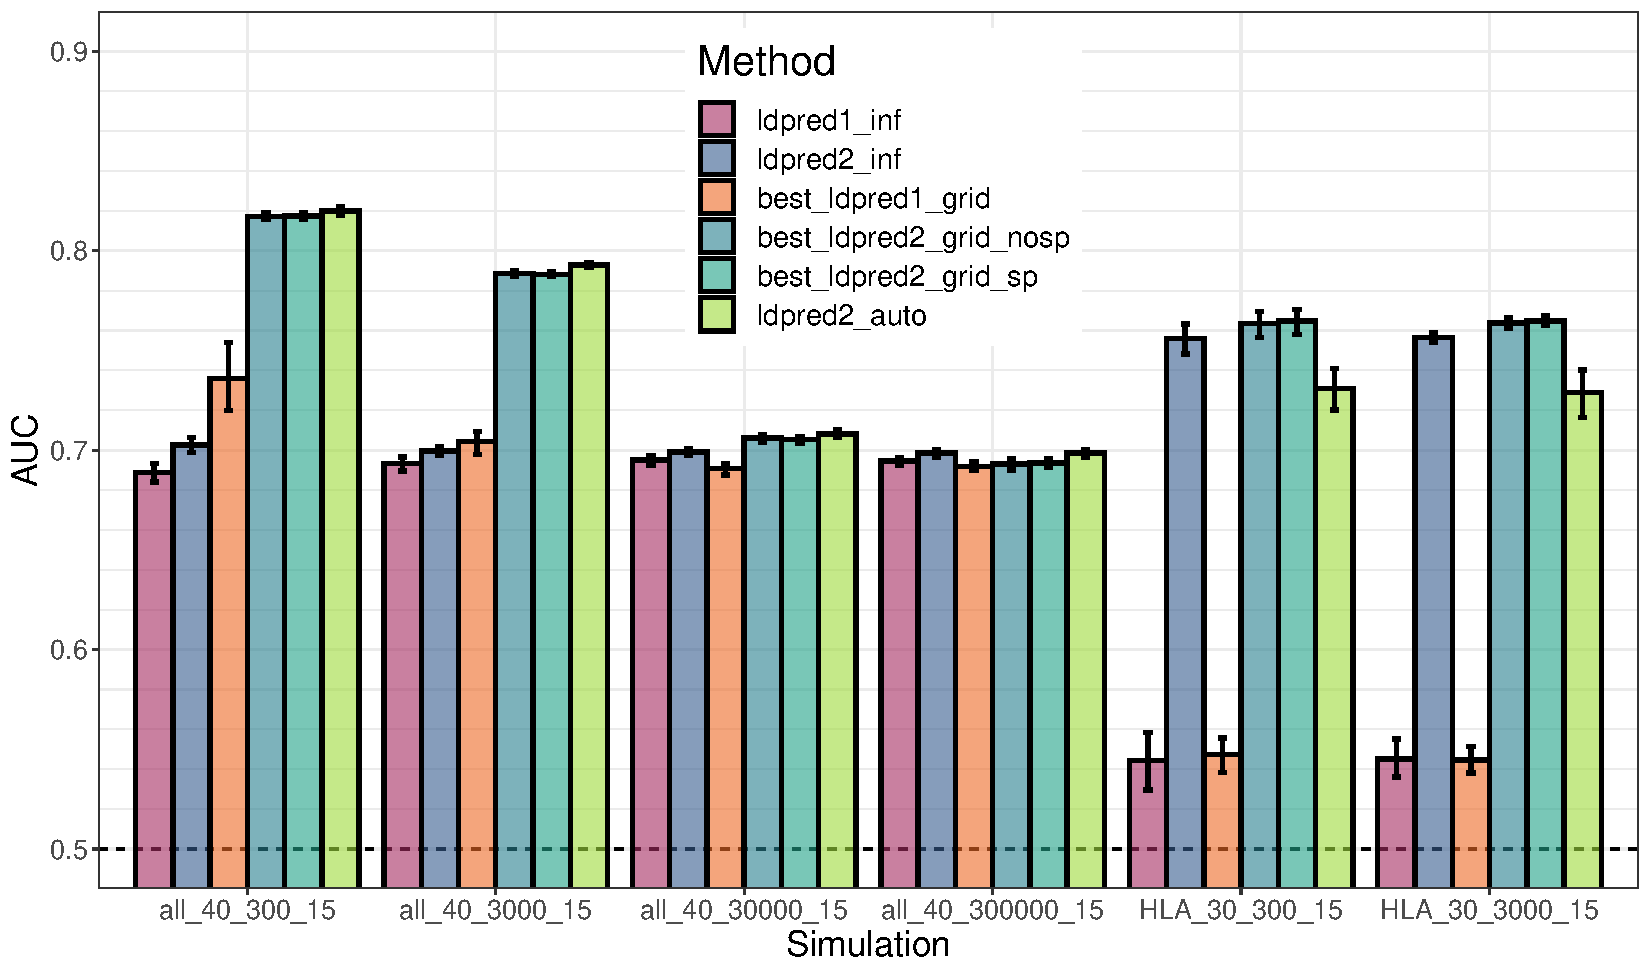
\includegraphics[width=0.85\textwidth]{AUC-simu}}
\caption{Six variants of LDpred are compared (two variants of LDpred1 in magenta and orange, and four variants of LDpred2 in blue and green colors) in the six simulation scenarios. 
Scenarios are named in 4 parts separated by underscores: 1) ``all'' means that causal variants are randomly sampled anywhere on the genome while ``HLA'' means that they are sampled in the HLA region of chromosome 6 (25.5-33.5 Mb); 2) the heritability (in \%); 3) the number of causal variants; 4) the prevalence (in \%).
Bars present the mean and 95\% CI of 10,000 non-parametric bootstrap replicates of the mean AUC of 10 simulations for each scenario. 
%See corresponding values in table S1.
}
\label{fig:AUC-simu}
\end{figure}

\subsection*{Real data}

Figure \ref{fig:AUC-real} presents the results of real data applications comparing LDpred1 (v1.0.0 as implemented by \cite{vilhjalmsson2015modeling}) with the new LDpred2 (as implemented in R package bigsnpr). 
Eight case-control phenotypes are used, summarized in table \ref{tab:sumstats}.
For T1D, T2D, BRCA and PRCA, all main LDpred2 models perform much better than LDpred1.
For example, for BRCA, AUC improves from 58.9\% with LDpred1 to 64.6\% with LDpred2, and from 57.4\% to 77.0\% for T1D.
These improvements are also significant for MDD and CAD, albeit to a lesser extend. 
For Asthma and RA, predictive performance of LDpred1 and LDpred2 are similar.
As in simulations, the sparse version of LDpred2 performs similarly to the non-sparse version.
Moreover, LDpred2-auto also performs well, and even better than LDpred2-grid for PRCA with an improvement from an AUC of 68.2\% to 70.2\%.
When comparing to other PGS methods, we only report the best LDpred2 model (chosen using the validation set) and LDpred2-auto. 
LDpred2 performs best for Asthma, RA, T1D and TD2, while lassosum performs best for BRCA, CAD, MDD and PRCA (Figure \ref{fig:AUC-all}).
We note that LDpred2-auto usually performs even better than LDpred-best (Figure \ref{fig:AUC-all}). This means that choosing the best LDpred model per chromosome leads to overfitting in the validation set, which does not transfer favorably when evaluating prediction performance in the test set.

%% FIGURE 2 HERE
\begin{figure}[htbp]
\centerline{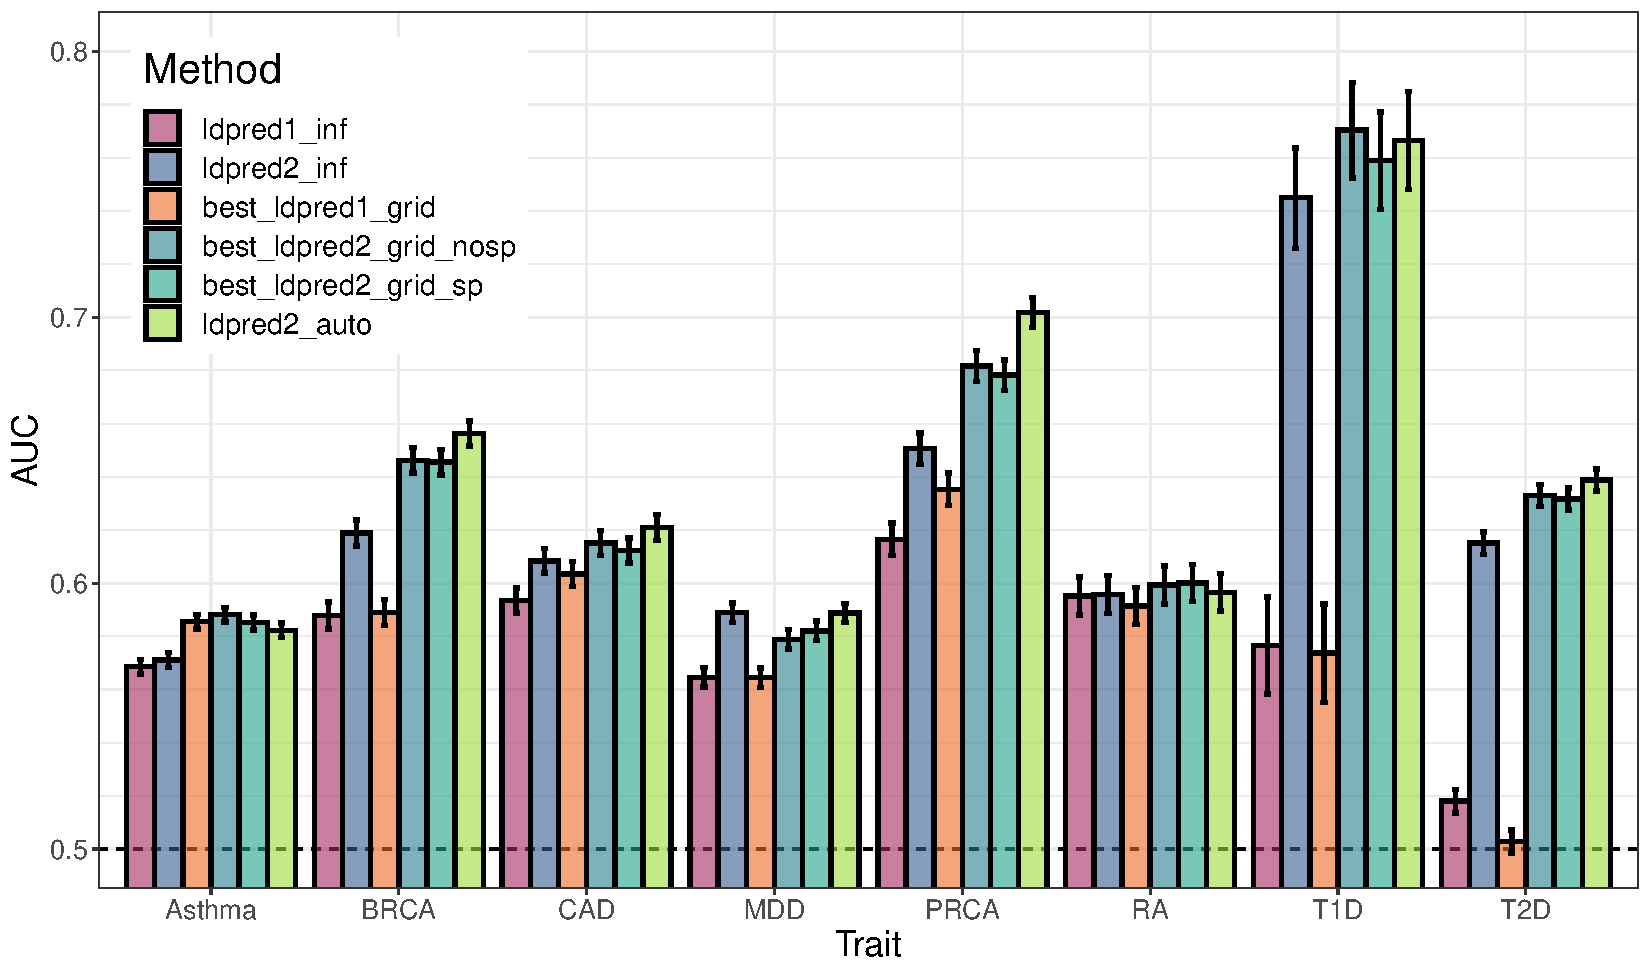
\includegraphics[width=0.85\textwidth]{AUC-real}}
\caption{Six variants of LDpred are compared (two variants of LDpred1 in magenta and orange, and four variants of LDpred2 in blue and green colors) in the real data applications using published external summary statistics.
Bars present AUC values on the test set of UKBB (mean and 95\% CI from 10,000 bootstrap samples).
%See corresponding values in table S2.
}
\label{fig:AUC-real}
\end{figure}

%% FIGURE 3 HERE
\begin{figure}[htbp]
\centerline{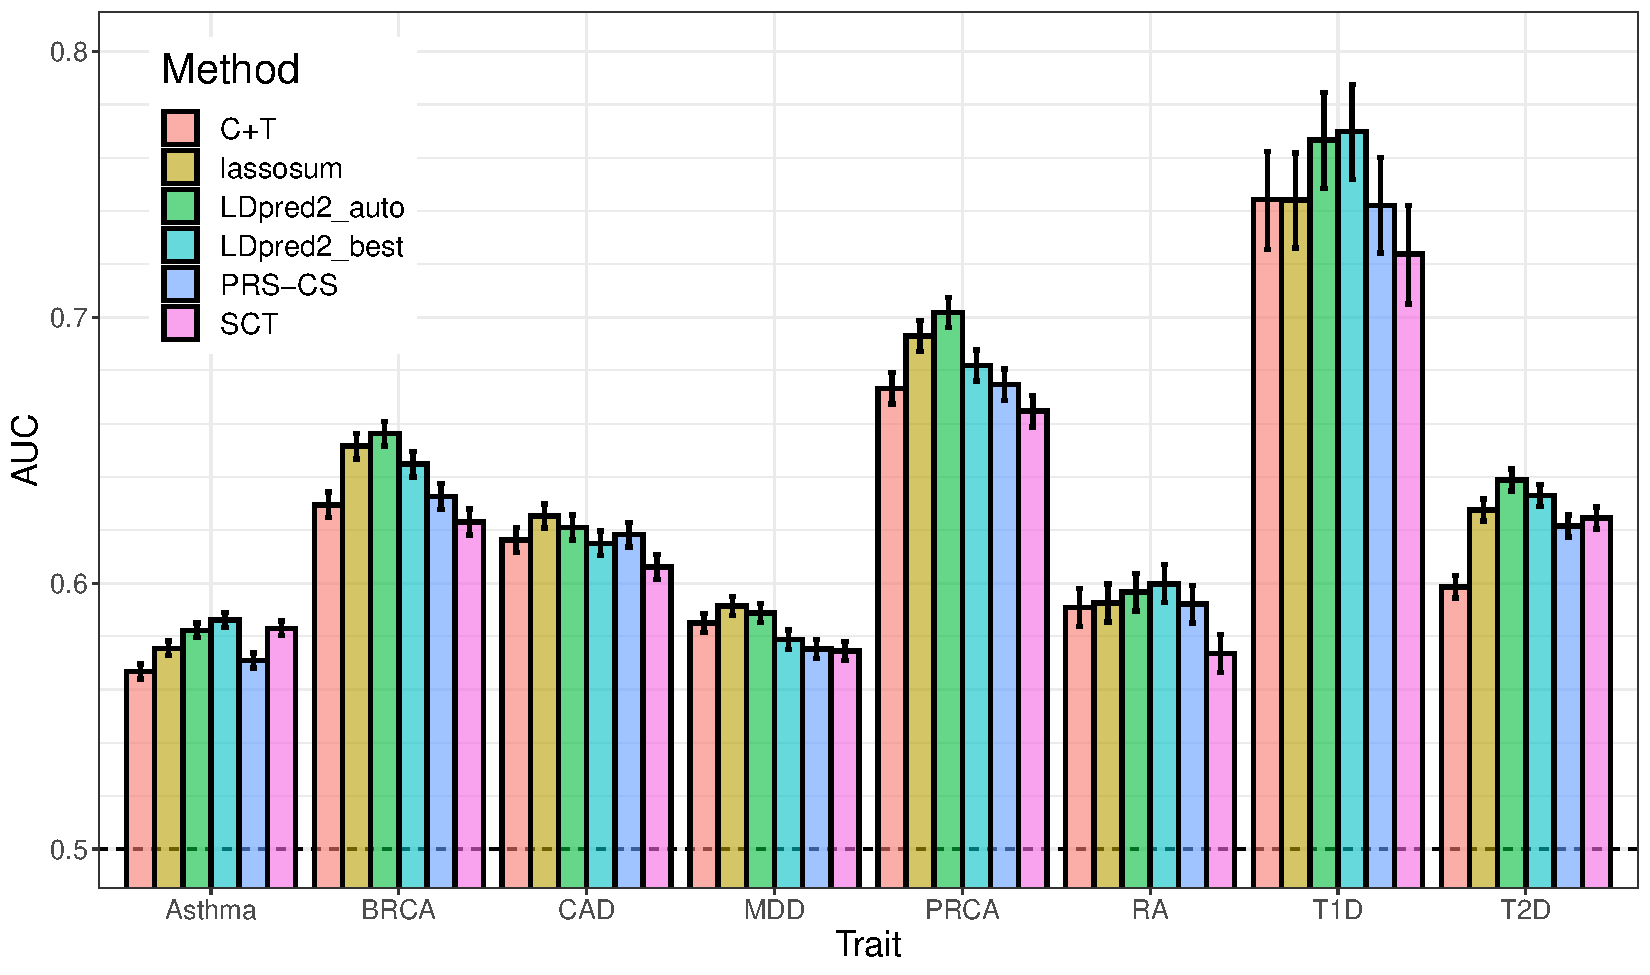
\includegraphics[width=0.85\textwidth]{AUC-all}}
\caption{LDpred2 is compared with C+T, SCT, lassosum and PRS-CS in the real data applications using published external summary statistics.
Bars present AUC values on the test set of UKBB (mean and 95\% CI from 10,000 bootstrap samples).
%See corresponding values in table S2.
}
\label{fig:AUC-all}
\end{figure}

%%%%%%%%%%%%%%%%%%%%%%%%%%%%%%%%%%%%%%%%%%%%%%%%%%%%%%%%%%%%%%%%%%%%%%%%%%%%%%%%

\section{Discussion}

The previous version of LDpred has been widely used and has the potential to provide polygenic models with good predictive performance \cite[]{khera2018genome}. 
Yet, it has instability issues that have been pointed out \cite[]{marquez2018modeling,lloyd2019improved} and likely contributed to discrepancies in reported prediction accuracies \cite[]{choi2019prsice,ge2019polygenic}.
We have therefore implemented a new version of LDpred, LDpred2, to address these issues and improve its computational efficiency.
We show that LDpred2 is more stable and provides higher predictive performance than LDpred1, particularly when handling long-range LD regions or less polygenic traits.
We hypothesize that LDpred1 does not use a LD window size that is large enough to account for long-range LD such as in the HLA region.
In LDpred2, we use a window size of 3 cM, which is larger than the default value used in LDpred1.
This enables LDpred2 to work well even when causal variants are located in long-range LD regions.
%We hypothesize that using a larger LD window explains the 5 real traits where LDpred2 performs much better than LDpred1, especially because LDpred2-inf performs better than LDpred1-inf.
We argue against removing these regions as sometimes suggested in the literature \cite[]{marquez2018modeling,lloyd2019improved}. 
Indeed, these regions, especially the HLA region, contain lots of variants associated with many traits, and are therefore very useful for prediction.

In LDpred2, we also expand the grid of hyper-parameters examined with now more values for $p$ (21 instead of 7 by default in LDpred1) and for $h^2$ (3 instead of 1).
When testing the grid of hyper-parameters of $p$ and $h^2$, we also allow for testing an option to enable sparse models in LDpred2 (see below).
Overall, we test a grid of 126 different values in LDpred2 instead of 7 in LDpred1.
We also use a larger window size for computing correlations between variants (see above), yet LDpred2 is still as fast as LDpred1.
The efficiency of LDpred2 is achieved through an efficient parallel implementation in C++. The parallelization is performed on the grid of hyper-parameters, but can also be performed chromosome-wise, as each chromosome is processed independently in LDpred2 (see Methods).
Efficient parallelization is possible because we developed an on-disk sparse matrix format accessed using memory mapping in R package bigsparser. 
As an example, it takes around less than three hours in total to run LDpred2-inf, LDpred2-grid (126 hyper-parameter values parallelized over 8 cores) and LDpred2-auto (30 initial values for $p$ parallelized over 8 cores) for a chromosome with 100,000 variants.
It takes 11 minutes to pre-compute the LD matrix for 10,000 individuals and 100,000 variants (using 16 cores).

LDpred2 also extends the original LDpred model in two ways.
First, we provide a sparse option in LDpred2-grid which provides models that truly encourage sparsity, in contrast to LDpred1 which outputs very small non-zero effect sizes \cite[]{cecile2019polygenic}.
In practice, the sparse version od LDpred2 can drastically reduce the number of variants used in the PGS without impacting its predictive performance, as opposed to discarding the smallest effects after having run LDpred (as shown in \cite{bolli2019software}).
%This sparse model performs equally well as the non-sparse model, therefore we encourage users to test it in the grid and to choose it if it performs better or equally well as the non-sparse model.
The second extension is LDpred2-auto, which automatically estimates values for hyper-parameters $p$ and $h^2$, therefore it does not require a validation step to choose hyper-parameters, making it an attractive option in many applications. 
LDpred2-auto performs equally well as other LDpred2 models in simulations. It also performs very well in real data applications, provided that some quality control is performed on summary statistics (see Supplementary Note).
This quality control aims at ensuring that effects are transferable from the external GWAS summary statistics to the data where PGS are computed.

In conclusion, we have shown that LDpred2 provides a better, faster and more robust implementation of the LDpred model.
LDpred2 also performs favorably when comparing it to recently derived methods that showed higher predictive performance compared to the previous version of LDpred. 
Indeed, LDpred2 (especially LDpred2-auto) provides the highest predictive performance for almost all the real traits tested here, and very good predictive performance for the others.
Note that the comparison may not be totally fair for C+T and SCT, as we use the same set of variants for all methods. 
Indeed, one should probably use a set enriched for statistically significant variants in C+T and SCT \cite[]{prive2019making}.
Further investigation is needed to determine whether doing so would be beneficial for other methods such as LDpred2, lassosum and PRS-CS, or detrimental as it may break some of the assumptions behind their respective models.
For now, we recommend using the same HapMap3 variants used in PRS-CS and used here.
Investigating variant selection for LDpred2 and other methods is a direction of future research for us.


%%%%%%%%%%%%%%%%%%%%%%%%%%%%%%%%%%%%%%%%%%%%%%%%%%%%%%%%%%%%%%%%%%%%%%%%%%%%%%%%

\section{Methods}

\subsection*{Simulation analyses}

We use the UK Biobank data for both real data analyses and simulations \cite[]{bycroft2018uk}. 
We restrict individuals to the ones used for computing the principal components (PCs) in the UK Biobank; these individuals are unrelated and have passed some quality control \cite[]{bycroft2018uk}.
To get a set of genetically homogeneous individuals, we compute a robust Mahalanobis distance based on the first 16 PCs and further restrict individuals to those within a log-distance of 5 \cite[]{prive2020efficient}.
We restrict variants to the HapMap3 variants used in PRS-CS \cite[]{ge2019polygenic}.
This results in 362,320 individuals and 1,117,493 variants.
We use 10,000 individuals as validation set for choosing optimal hyper-parameters and for computing correlations between variants (LD matrix $\boldsymbol{R}$). 
We use 300,000 other individuals for running logistic GWAS to create summary statistics.
We use the remaining 52,320 individuals as test set for evaluating models.

We simulate binary phenotypes with a heritability of $h^2=0.4$ (or 0.3)  using a Liability Threshold Model (LTM) with a prevalence of 15\% \cite[]{falconer1965inheritance}. 
We vary the number of causal variants (300, 3000, 30,000, or 300,000) to match a range of genetic architectures from low to high polygenicity.
Liability scores are computed from a model with additive effects only: we compute the liability score of the $i$-th individual as \(y_i = \sum_{j\in S_\text{causal}} w_j \widetilde{G}_{i,j} + \epsilon_i,\) where $S_\text{causal}$ is the set of causal variants, $w_j$ are weights generated from a Gaussian distribution $N(0, h^2 / \vert S_\text{causal} \vert)$, $G_{i,j}$ is the allele count of individual $i$ for variant $j$, $\widetilde{G}_{i,j}$ corresponds to its standardized version (zero mean and unit variance), and $\epsilon_i$ follows a Gaussian distribution $N(0, 1 - h^2)$.
Causal variants are chosen randomly anywhere on the genome. 
We design two other simulation scenarios with 300 or 3000 causal variants randomly chosen in the HLA region (chromosome 6, 25.5-33.5 Mb).
Both parts of the $y_i$'s are scaled such that the variance of the genetic liability is exactly $h^2$ and the variance of the total liability is exactly $1$. 
Such simulation of phenotypes based on real genotypes is implemented in function \texttt{snp\_simuPheno} of R package bigsnpr.
Each simulation scenario is repeated 10 times and averages of the Area Under the ROC Curve (AUC) are reported. 


\subsection*{Real data analyses}

We use the same data as in the simulation analyses. We use the same 10,000 individuals as validation set, and use the remaining 352,320 individuals as test set.
We use external published GWAS summary statistics listed in table \ref{tab:sumstats}.
We defined phenotypes as in \cite{prive2019making}. Some quality control is applied to summary statistics (see Supplementary Note).
For more details, please refer to our R code (Software and code availability section).

%% TABLE 1 HERE
\begin{table}[h]
	\centering
	\begin{tabular}{|l|c|c|c|c|}
		\hline
		Trait & GWAS citation & GWAS sample size & GWAS \#variants \\
		\hline
		Breast cancer (BRCA) & \cite{michailidou2017association} & 137,045 / 119,078 & 11,792,542 \\
		Rheumatoid arthritis (RA) & \cite{okada2014genetics} & ~~29,880 / ~~73,758 & ~~9,739,303 \\
		Type 1 diabetes (T1D) & \cite{censin2017childhood} & ~~~~~5913 / ~~~~~8828  & ~~8,996,866 \\
		Type 2 diabetes (T2D) & \cite{scott2017expanded} & ~~26,676 / 132,532 & 12,056,346 \\
		Prostate cancer (PRCA) & \cite{schumacher2018association} & ~~79,148 / ~~61,106 & 20,370,946 \\
		Depression (MDD) & \cite{wray2018genome} & ~~59,851 / 113,154 & 13,554,550 \\
		Coronary artery disease (CAD) & \cite{nikpay2015comprehensive} & ~~60,801 / 123,504 & ~~9,455,778 \\
		Asthma & \cite{demenais2018multiancestry} & ~~19,954 / 107,715 & ~~2,001,280 \\
		\hline
	\end{tabular}
	\caption{Summary of external GWAS summary statistics used. The GWAS sample size is the number of cases / controls in the GWAS. \label{tab:sumstats}}
\end{table}

In real data applications, we first compare all four LDpred2 models to the two LDpred1 models.
Then, we compare the best of the four LDpred2 models (chosen using the validation set, and for each chromosome) and LDpred2-auto to four other methods: Clumping and Thresholding (C+T), Stacked C+T (SCT), lassosum and PRS-CS \cite[]{prive2019making,mak2017polygenic,ge2019polygenic}.
For C+T and SCT, we use a large grid of hyper-parameters as in \cite{prive2019making}.
For lassosum, we use the default grid of hyper-parameters $s$ and $\lambda$. 
Finally, for PRS-CS, we use the grid $\{10^{-6}, 10^{-5}, \dots, 1\}$ for the global scaling hyper-parameter $\Phi$, and the default values for hyper-parameters $a$ and $b$. 


\subsection*{From marginal effects to joint effects}

In this section, we explain how we can obtain joint effects from summary statistics (marginal effects) and a correlation matrix $\boldsymbol{R}$.
Let us denote by $\boldsymbol{S}$ the diagonal matrix with standard deviations of the $m$ variants, $\boldsymbol{C_n} = \boldsymbol{I_n} - \boldsymbol{1} \boldsymbol{1}^T / n$ the centering matrix, $\boldsymbol{G}$ the genotype matrix of $n$ individuals and $m$ variants, and $\boldsymbol{y}$ the phenotype vector for $n$ individuals.

When solving a joint model with all variants and an intercept ${\alpha}$, the joint effects $\boldsymbol{\gamma}_{\text{joint}}$ are obtained by solving
\[\begin{bmatrix} \hat{\alpha} \\ \boldsymbol{\hat{\gamma}_{\text{joint}}} \end{bmatrix} = \left(\begin{bmatrix} \boldsymbol{1} & \boldsymbol{G} \end{bmatrix}^T \begin{bmatrix} \boldsymbol{1} & \boldsymbol{G} \end{bmatrix}\right)^{-1} \begin{bmatrix} \boldsymbol{1} & \boldsymbol{G} \end{bmatrix}^T \boldsymbol{y} ~.\]
Using the Woodburry formula, we get 
\[\boldsymbol{\hat{\gamma}_{\text{joint}}} = (\boldsymbol{G}^T \boldsymbol{C_n} \boldsymbol{G})^{-1} \boldsymbol{G}^T \boldsymbol{C_n} \boldsymbol{y} ~.\]
When fitting each variant separately in GWAS, the marginal effects (assuming no covariate) simplify to 
\[\boldsymbol{\hat{\gamma}_{\text{marg}}} = \dfrac{1}{n-1} \boldsymbol{S}^{-2} \boldsymbol{G}^T \boldsymbol{C_n} \boldsymbol{y} ~.\] 
We further note that the correlation matrix of $\boldsymbol{G}$ is \(\boldsymbol{R} =  \dfrac{1}{n-1} \boldsymbol{S}^{-1} \boldsymbol{G}^T \boldsymbol{C_n} \boldsymbol{G}  \boldsymbol{S}^{-1}\).
Then we get 
\begin{equation}\label{eq:joint}
\boldsymbol{\hat{\gamma}_{\text{joint}}} = \boldsymbol{S}^{-1} \boldsymbol{R}^{-1} \boldsymbol{S} \boldsymbol{\hat{\gamma}_{\text{marg}}} ~.
\end{equation}
In practice, the correlation matrix $\boldsymbol{R}$ is usually not available but is computed from another dataset. 
Also note that $\boldsymbol{\gamma}$ are the effects on the allele scale while we denote by $\boldsymbol{\beta} = \boldsymbol{S} \boldsymbol{\gamma}$ the effects of the scaled genotypes.

For the marginal effect $\hat{\gamma}_j$ of variant $j$, let us denote by $\boldsymbol{\breve{y}}$ and $\boldsymbol{\breve{G}_j}$ the vectors of phenotypes and genotypes for variant $j$ residualized from $K$ covariates, e.g.\ centering them.
Then,
\[\left(\text{se}(\hat{\gamma}_j)\right)^2 = \dfrac{(\boldsymbol{\breve{y}} - \hat{\gamma}_j \boldsymbol{\breve{G}_j})^T (\boldsymbol{\breve{y}} - \hat{\gamma}_j \boldsymbol{\breve{G}_j})}{(n - K - 1) ~ \boldsymbol{\breve{G}_j}^T \boldsymbol{\breve{G}_j}} \approx \dfrac{\boldsymbol{\breve{y}}^T \boldsymbol{\breve{y}}}{n ~ \boldsymbol{\breve{G}_j}^T \boldsymbol{\breve{G}_j}} \approx \dfrac{\text{var}(\boldsymbol{y})}{n ~ \text{var}(\boldsymbol{G_j})} ~.\]
The first approximation is possible because $\hat{\gamma}_j$ is expected to be small, while the second approximation assumes that the effects from covariates are small. 
Thus, we can derive $\text{sd}(\boldsymbol{G_j}) \approx \dfrac{\text{sd}(\boldsymbol{y})}{\text{se}(\hat{\gamma}_j) ~ \sqrt{n}}$ and then $\left(\text{sd}(\boldsymbol{G_j}) ~ \hat{\gamma}_j\right) \approx \dfrac{\hat{\gamma}_j}{\text{se}(\hat{\gamma}_j)} \dfrac{\text{sd}(\boldsymbol{y})}{\sqrt{n}}$.
Let us go back to equation \ref{eq:joint}. 
As $\text{sd}(\boldsymbol{y})$ is the same for all variants, it is cancelled out by $\boldsymbol{S}^{-1}$ and $\boldsymbol{S}$, therefore we can assume that $\text{var}(\boldsymbol{y}) = 1$. 
It justifies the use of the Z-scores ($\hat{\gamma}_j ~/~ \text{se}(\hat{\gamma}_j)$) divided by $\sqrt{n}$ as input for LDpred (first line of algorithm \ref{algo:ldpred}). Then, the effect sizes that LDpred outputs need to be scaled back by multiplying by $\left(\text{se}(\hat{\gamma}_j) ~ \sqrt{n}\right)$ (last line of algorithm \ref{algo:ldpred}).
In LDpred2, we allow for having different $n_j$ for different variants. 
Note that LDpred1 and other similar methods scale the output dividing by the standard deviation of genotypes. This is correct when $\text{var}(\boldsymbol{y}) = 1$ only.
In the case of binary phenotypes, the approximation of the standard deviations is slightly different (see Supplementary Note).




\subsection*{Overview of LDpred model}

LDpred assumes the following model for effect sizes,
\begin{equation}\label{eq:model}
\beta_j = S_{j,j} \gamma_j \sim \left\{
\begin{array}{ll}
\mathcal N\left(0, \dfrac{h^2}{M p}\right) & \mbox{with probability $p$,} \\
0 & \mbox{otherwise,}
\end{array}
\right.
\end{equation}
where $p$ is the proportion of causal variants, $M$ the number of variants and $h^2$ the (SNP) heritability.
\cite{vilhjalmsson2015modeling} estimate $h^2$ using constrained LD score regression (intercept fixed to 1) and recommend testing a grid of hyper-parameter values for $p$ (1, 0.3, 0.1, 0.03, 0.01, 0.003 and 0.001).

\newcommand{\hmpn}{\dfrac{h^2}{M p} + \dfrac{1}{n}}
\newcommand{\phmpn}{\dfrac{p}{\sqrt{\hmpn}}}
\newcommand{\betahmpn}{\dfrac{\tilde{\beta}_j^2}{\hmpn}}

To estimate effect sizes $\beta_j$, \cite{vilhjalmsson2015modeling} use a Gibbs sampler, as described in algorithm \ref{algo:ldpred}.
First, the residualized marginal effect for variant $j$ is computed as
\begin{equation}\label{eq:beta_res}
\tilde{\beta}_j = \hat{\beta}_j - \boldsymbol{\beta_{-j}}^T \boldsymbol{R_{-j, j}}
\end{equation}
where $\boldsymbol{R_{-j, j}}$ is the $j$-th column without the  $j$-th row of the correlation matrix, $\boldsymbol{\hat{\beta}}$ is the vector of marginal effect sizes, $\boldsymbol{{\beta}}$ is the vector of current effect sizes in the Gibbs sampler, and $\boldsymbol{\beta_{-j}}$ is $\boldsymbol{\beta}$ without the $j$-th element. 
Then, the probability that variant $j$ is causal is computed as 
\[\bar{p}_j = P\left(\beta_j \sim \mathcal N(\cdot,\cdot) ~|~ \tilde{\beta}_j\right) = \dfrac{\phmpn \exp\left\lbrace-\dfrac{1}{2} \betahmpn\right\rbrace}{\phmpn \exp\left\lbrace-\dfrac{1}{2} \betahmpn\right\rbrace + \dfrac{1-p}{\sqrt{\dfrac{1}{n}}} \exp\left\lbrace-\dfrac{1}{2} \dfrac{\tilde{\beta}_j^2}{\dfrac{1}{n}}\right\rbrace}~,\]
which we rewrite as
\begin{equation}
\bar{p}_j = \dfrac{1}{1 + \dfrac{1-p}{p} \sqrt{1 + \dfrac{n h^2}{Mp}} \exp\left\lbrace-\dfrac{1}{2} \dfrac{n \tilde{\beta}_j^2}{1 + \dfrac{Mp}{n h^2}}\right\rbrace}~.\label{eq:postp}
\end{equation}
Computing $\bar{p}_j$ using the second expression is important to avoid numerical issues when $\left(n \tilde{\beta}_j^2\right)$ is large.

Then, $\beta_j$ is sampled according to
\begin{equation}\label{eg:random_beta}
\beta_j ~|~ \tilde{\beta}_j \sim \left\{
\begin{array}{ll}
\mathcal N\left(\dfrac{1}{1 + \dfrac{M p}{n h^2}} \tilde{\beta}_j, \dfrac{1}{1 + \dfrac{M p}{n h^2}}\dfrac{1}{n}\right) & \mbox{with probability $\bar{p}_j$,} \\
0 & \mbox{otherwise.}
\end{array}
\right.
\end{equation}

Therefore, the posterior mean of $\beta_j ~|~ \tilde{\beta}_j$ is given by 
\begin{equation}\label{eg:post_beta}
\omega_j = \dfrac{\bar{p}_j \tilde{\beta}_j}{1 + \dfrac{M p}{n h^2}} ~.
\end{equation}

\begin{algorithm}[H]
\caption{LDpred, with hyper-parameters $p$ and $h^2$, LD matrix $\boldsymbol{R}$ and summary statistics $\boldsymbol{\hat{\gamma}}$, $\boldsymbol{\text{se}(\hat{\gamma})}$ and $\boldsymbol{n}$}\label{algo:ldpred}
\begin{algorithmic}[1]
	\State $\boldsymbol{\hat{\beta}} \gets \dfrac{\boldsymbol{\hat{\gamma}}}{\boldsymbol{\text{se}(\hat{\gamma})} \cdot \sqrt{\boldsymbol{n}}}$ \Comment{Initialization of scaled marginal effects (see previous section)}
	\State $\boldsymbol{\Omega} \gets \boldsymbol{0}$ \Comment{Initialization of posterior means}
	\For {$k=1,\ldots,N_\text{burn-in} + N_\text{iter}$} \Comment{Gibbs iterations}
	\For {each variant $j$} \Comment{All variants}
	\State Compute $\tilde{\beta}_j$ according to \eqref{eq:beta_res}
	\State Compute $\bar{p}_j$ according to \eqref{eq:postp}
	\State Sample $\beta_j$ according to \eqref{eg:random_beta}
	\State Compute $\omega_j$ according to \eqref{eg:post_beta}
	\EndFor
	\If {$k > N_\text{burn-in}$} 
	\State $\boldsymbol{\Omega} \gets \boldsymbol{\Omega} + \boldsymbol{\omega}$ 
	\EndIf
	\EndFor
	\State $\boldsymbol{\Omega} \gets \boldsymbol{\Omega} /  N_\text{iter}$ \Comment{Average of all $\boldsymbol{\omega}$ after burn-in}
	\State Return $\boldsymbol{\Omega} \cdot  \boldsymbol{\text{se}(\hat{\gamma})} \cdot \sqrt{\boldsymbol{n}}$ \Comment{Return posterior means, scaled back (see previous section)}
\end{algorithmic} 
\end{algorithm}


\subsection*{New LDpred2 models}

LDpred2 comes with two extensions of the LDpred model.

The first extension consists in estimating $p$ and $h^2$ within the model, as opposed to testing several values of $p$ and estimating $h^2$ using constrained LD score regression \cite[]{bulik2015ld}. This makes LDpred2-auto a method free of hyper-parameters which can therefore be applied directly to data without the need of a validation dataset to choose best-performing hyper-parameters.
To estimate $p$, we count the number of causal variants (i.e.\ $M_c = \sum_j(\beta_j \neq 0)$ in equation \ref{eg:random_beta}). 
We can assume that $M_c \sim \text{Binom}(M, p)$, so if we place a prior $p \sim \text{Beta}(1, 1) \equiv \mathcal{U}(0, 1)$, we can sample $p$ from the posterior $p \sim \text{Beta}(1 + M_c, 1 + M - M_c)$.
Due to complexity reasons, we could not derive a Bayesian estimator of $h^2$. Instead, we estimate $h^2 = \boldsymbol{\beta}^T \boldsymbol{R} \boldsymbol{\beta}$, where $\boldsymbol{R}$ is the correlation matrix.
These parameters $p$ and $h^2$ are updated after the inner loop in algorithm \ref{algo:ldpred}, then these new values are used in the next iteration of the outer loop.

The second extension, LDpred2-sparse, aims at providing sparse effect size estimates, i.e.\ some resulting effects are exactly 0.
When the sparse solution is sought and when $\bar{p}_j < p$, we set $\beta_j$ and $\omega_j$ to 0 (lines 6-8 of algorithm \ref{algo:ldpred}).
Note that LDpred2-auto does not have a sparse option, but it is possible to run LDpred2-sparse with the estimates of $p$ and $h^2$ from LDpred2-auto.

When running LDpred2-grid, we test a grid of hyper-parameters with $p$ from a sequence of 21 values from $10^{-5}$ to $1$ on a log-scale; $h^2$ within $\{0.7, 1, 1.4\} \cdot h^2_\text{LDSC}$, where $h^2_\text{LDSC}$ is the heritability estimate from the constrained LD score regression \cite{bulik2015ld}; and whether sparsity is enabled or not.
In total, this grid is of size $21 \times 3 \times 2 = 126$.
When running LDpred2-auto, we run it 30 times with $h^2_\text{LDSC}$ as initial value for $h^2$ and a sequence of 30 values from $10^{-4}$ to $0.9$ on a log-scale as initial values for $p$.
Running many Gibbs chains aims at checking that models did not diverge (and hopefully converged).
As a criterion for non-divergence, we compute the standard deviations of the resulting predictors from the 30 models, keep only those within 3 median absolute deviations from their median, and average the remaining vectors of effects as final effect sizes for the ``auto'' version.

\subsection*{New strategy for local correlation}

There is a window size parameter that needs to be set in LDpred; for a given variant, correlations with other variants outside of this window are assumed to be 0.
The recommended value for this window (in number of variants) has been to use the total number of variants divided by 3000, which corresponds to a window radius of around 2 Mb \cite[]{vilhjalmsson2015modeling}.
We have come to the conclusion that this window size is not large enough. Indeed, the human leukocyte antigen (HLA) region of chromosome 6 is 8 Mb long \cite[]{price2008long}. 
Using a window of 8Mb would be computationally and memory inefficient.
Instead, we propose to use genetic distances. Genome-wide, 1 Mb corresponds on average to 1 cM. Yet, the HLA region is only 3 cM long (vs.\ 8 Mb long).
Therefore, genetic distances enable to capture the same LD using a globally smaller window.
We provide function \texttt{snp\_asGeneticPos} in package bignspr to easily interpolate physical positions (in bp) to genetic positions (in cM).
We recommend to use genetic positions and to use a size parameter of 3 cM when computing the correlation between variants for LDpred2. 
Note that, in the code, we use \texttt{size = 3 / 1000} since parameter \texttt{size} is internally multiplied by 1000 in the bigsnpr functions.

\subsection*{New strategy for running LDpred2}\label{sec:bychr}

We run LDpred2 per chromosome.
Even if it is possible to run LDpred2 genome-wide, this approach has two drawbacks. First, it can be memory and computationally demanding to do so. For around one million (1M) variants, storing the 1M$\times$1M sparse correlation matrix takes more than 32 GB of memory. 
Doubling to 2M variants would require 128 GB of RAM to store the matrix.
Second, as noted in \cite{prive2019making}, it may be beneficial to assume that the architecture of traits is different for different chromosomes.
For example, chromosome 6 clearly encompasses a larger proportion of the heritability of autoimmune diseases compared to other chromosomes \cite[]{shi2016contrasting}.
Assuming the same model for genetic effects genome-wide could result in model misspecification, which would lead to suboptimal predictive performance.
Moreover, since the inverse of a block-diagonal matrix is formed from the inverse of each block, it should be safe to run LDpred2 for each chromosome and then combine the results. 
To choose the best LDpred2 model, one can choose the best model according to their preferred criterion (e.g. max AUC). 
Here, we use the Z-Score from the regression of the phenotype by the PRS since we have found it more robust than using the AUC.


%%%%%%%%%%%%%%%%%%%%%%%%%%%%%%%%%%%%%%%%%%%%%%%%%%%%%%%%%%%%%%%%%%%%%%%%%%%%%%%%

\clearpage
%\vspace*{5em}

\section*{Software and code availability}

%[TODO: EXPORT CODE FROM CLUSTER] 

All code used for this paper is available at \url{https://github.com/privefl/paper-ldpred2/tree/master/code}.
The newest version of R package bigsnpr can be installed from GitHub (see \url{https://github.com/privefl/bigsnpr}).
A tutorial on the steps to run LDpred2 using some small example data is available at \url{https://privefl.github.io/bigsnpr/articles/LDpred2.html}. 

\section*{Acknowledgements}

Authors thank Yixuan Qiu for pointing to matrix-free solvers.
This research has been conducted using the UK Biobank Resource under Application Number 41181.
Authors would also like to thank GenomeDK and Aarhus University for providing computational resources and support that contributed to these research results.

\section*{Funding}

F.P. and B.V.\ are supported by the Danish National Research Foundation (Niels Bohr Professorship to Prof. John McGrath), and also acknowledge the Lundbeck Foundation Initiative for Integrative Psychiatric Research, iPSYCH (R248-2017-2003).

\section*{Declaration of Interests}

The authors declare no competing interests.

%%%%%%%%%%%%%%%%%%%%%%%%%%%%%%%%%%%%%%%%%%%%%%%%%%%%%%%%%%%%%%%%%%%%%%%%%%%%%%%%

\clearpage

\bibliographystyle{natbib}
\bibliography{refs}

%%%%%%%%%%%%%%%%%%%%%%%%%%%%%%%%%%%%%%%%%%%%%%%%%%%%%%%%%%%%%%%%%%%%%%%%%%%%%%%%


\end{document}
